% !TEX root = MasterPaper.tex
\chapter{臨場感を演出する集団ロボットの内部モデル}
\thispagestyle{fancy} % このページのみ
\lhead{}
\chead{}
\rhead{}
\lfoot{} 
\cfoot{\thepage}  
\rfoot{}
%

\section{モデルの概要}
\label{sec3.1}

本研究では,ユーザは感情表出を行うロボット集団と共に野球観戦を行う.その中で,提案ロボット集団はユーザへの感情伝播を行い,観戦時特有の臨場感を演出することを目的とする.

本節では,野球観戦するロボットが試合状況を読み取って感情表出するための内部モデルを紹介する.初めに試合状況を読み取る方法について,次にロボットの表出する感情の生成方法について述べる.

\subsection{試合状況の読み取り}
\label{sec3.1.1}    

本研究では,ロボットは観戦する試合状況を読み取ることで,試合展開に沿った感情表出を行う.試合状況は,プロ野球情報サイトである「キューステ!」で利用されている「勝利確率グラフ」を用いて読み取る\cite{kyusute}.ここで,勝利確率グラフとは,特定の試合状況(イニング・点差・走者・アウトカウント)において,チームにどれだけ勝利が見込まれるかをグラフ化したものである.

勝利確率グラフで示される値である勝利確率$Q$は,過去のチームの勝利数$S$と過去の同じ状況の場面数$N$を用いて式(\ref{eq:3.1})のように算出する.勝利数$S$と場面数$N$の値は,1995年~2018年の日本プロ野球公式記録を参照する.2019年4月5日に開催された阪神タイガース-広島東洋カープの試合の勝利確率グラフの例を図\ref{win_percent}に示す.試合開始の時点では両チームにそれぞれ50%の勝利確率が見込まれ,回が進み点差が開くほど優位なチームは100%に近付いていく.また,得点期待の高いシーンや,終盤の勝敗に直結するシーンなどは勝利確率が大きく変動する.

\vspace{1cm}
 \begin{figure}[H]
 \begin{center}
  \centering
  \includegraphics[width=13.5cm]{images/chapter3/winper.eps}
  \caption{勝利確率グラフ}
  \label{win_percent}
 \end{center}
\end{figure}


\begin{equation}
\label{eq:3.1}
 Q = \frac{S}{N}
\end{equation}





\subsection{感情の生成方法}
\label{sec3.1.2}

先行研究では,野球観戦において得点に対する期待感が高まる場面で,観戦者の歓声量が増加することが分かっている\cite{rinjyo3}.つまり,観戦者は勝利の確率が変動する場面で,感情を表出しているといえる.そのため,ロボットが観戦者と同じような場面で感情表出を行うことで,ユーザはロボットと違和感なく野球観戦をすることができると考えられる.

そこで,本研究では,ロボットは勝利確率グラフの増減値の幅$W$を用いて感情の生成を行う.増減値の幅$W$は現在の勝利確率$Q_{a}$と1つ前の勝利確率$Q_{b}$を用いて式(\ref{eq:3.2})のように定義する.
\begin{equation}
\label{eq:3.2}
 W = \frac{Q_{a}-Q_{b}}{100}
\end{equation}

現在のシーンの勝利確率を$Q_{a}$,1つ前のシーンの勝利確率を$Q_{b}$とし,100で割ることによって勝利確率の増減値の幅を算出する.

提案するロボットは,喜の感情と哀の感情の2種類の感情を生成する.$W$の符号によって感情の種類を決定し,$W > 0$なら喜の感情を,$W < 0$なら哀の感情を表出する.


\newpage

\section{実験環境}
\label{sec3.2}

実環境でのインタラクションにおいて,感情を表出するロボット集団を準備することや,リアルタイムでの勝利確率を取得することは困難であるため,本実験では仮想環境であるVR空間を用いて実験を行う.本研究では,採用しているバーチャルアバターをロボットと呼ぶ.ロボット集団と共に野球観戦を行うため,スポーツバーを模した空間をゲームエンジンであるUnityを用いて制作している\cite{unity}.

本実験では,観戦を行う場所としてスポーツバーを模した内装と,感情を表出するロボット集団を,Unity内のAsset storeにある有償のAssetを改変して使用している\cite{bar}\cite{lilrobot}.スポーツバーとロボット集団の外観を図\ref{sports_bar},図\ref{robot}に示す.

また,Unityで作成したVR空間を体験するためのデバイスとして,ヘッドマウントディスプレイ,ヘッドフォンを使用する.この機器は家庭用VRデバイスであるHTC VIVEを用いる\cite{vive}.

本実験で使用するヘッドフォン付きヘッドマウントディスプレイを図\ref{Vive}に示す.


\vspace{1cm}
 \begin{figure}[H]
 \begin{center}
  \centering
  \includegraphics[width=15cm]{images/chapter3/sports_bar.eps}
  \caption{実験環境}
  \label{sports_bar}
 \end{center}
\end{figure}


\newpage

\vspace{1cm}
 \begin{figure}[!h]
 \begin{center}
  \centering
  \includegraphics[width=15cm]{images/chapter3/robot.eps}
  \caption{ロボット集団}
  \label{robot}
 \end{center}
\end{figure}


\vspace{1cm}
 \begin{figure}[!h]
 \begin{center}
  \centering
  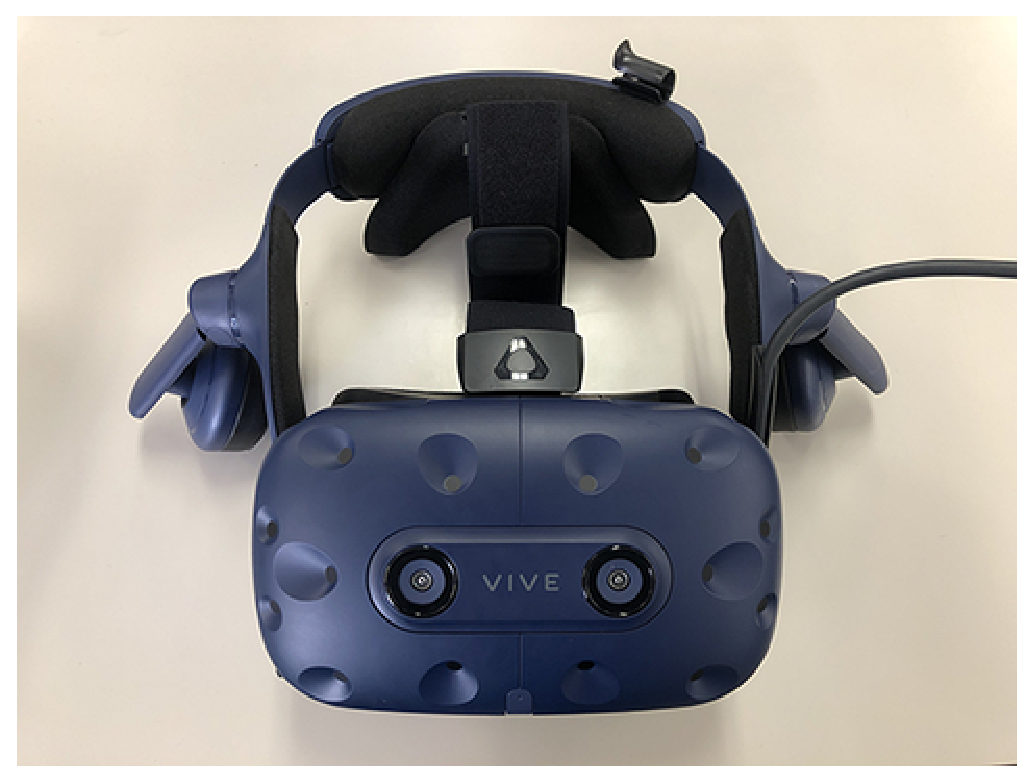
\includegraphics[width=12cm]{images/chapter3/Vive.eps}
  \caption{ヘッドマウントディスプレイ}
  \label{Vive}
 \end{center}
\end{figure}


\subsection{スポーツバーでの観戦}
\label{sec3.2.1}

実験中の画面の様子を図\ref{bar_scene}に示す.本実験では被験者とロボットのみで試合観戦を行う.共に試合観戦を行うロボット集団は,スポーツバーを模した空間上の席に着席して試合観戦を行う.

被験者はヘッドフォン付きヘッドマウントディスプレイを装着して着席し,その場から動かずにロボット集団と試合観戦を行う.図\ref{sports_bar}の前方にある4台のモニターに映し出される試合を観戦する.また,ヘッドマウントディスプレイによる映像だけでなく,ヘッドフォンからは観戦映像の音が流れている.このように,被験者は視覚情報と聴覚情報の2つを用いて試合観戦を行う.




\vspace{1cm}
 \begin{figure}[!h]
 \begin{center}
  \centering
  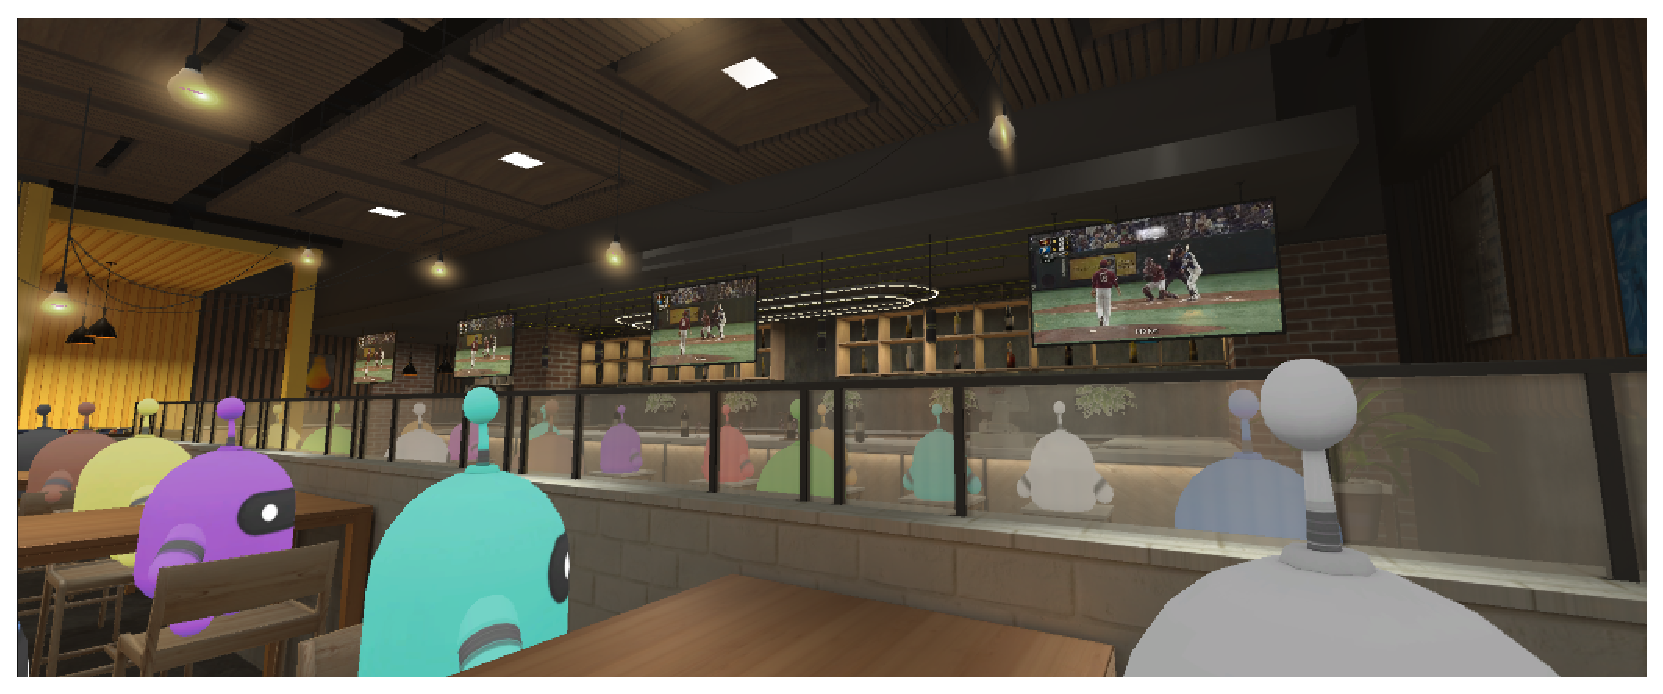
\includegraphics[width=15cm]{images/chapter3/bar_scene.eps}
  \caption{スポーツバーの様子}
  \label{bar_scene}
 \end{center}
\end{figure}



\newpage



\subsection{ロボット集団の動作}
\label{sec3.2.2}

被験者と共に試合観戦をするロボット集団は,感情表出しない状態(Idle状態),喜の感情表出,哀の感情表出を行う.

Idle状態では,ロボットは図\ref{Idle}の状態から,一定の周期でゆっくりと上下に反復運動を行う.この動作によって,人間の呼吸運動を再現する.また,各ロボットは,反復運動の速さを24回/分,27回/分,30回/分,33回/分,36回/分の5種類からランダムで設定されており,速さを変えることによってロボットの個性を設計している.

喜の感情表出は,図\ref{happy}のように,手を挙げながらジャンプする動作を繰り返すことで表出する.表出する感情の程度は,ジャンプする動作の速さを変更することで設計する.本実験では感情の程度を小,中,大の3種類に設定し,小なら30回/分,中なら50回/分,大なら70回/分の速さで感情表出を行う.

哀の感情表出は,図\ref{sad}のように,飛び上がって倒れこむ動作を繰り返すことで表出する.表出する感情の程度は,倒れこむ速さを変更することで設計する.喜の感情と同じく3段階の感情の程度を設定し,小なら12回/分,中なら15回/分,大なら20回/分の速さで感情表出を行う.


\vspace{1cm}
 \begin{figure}[!h]
 \begin{center}
  \centering
  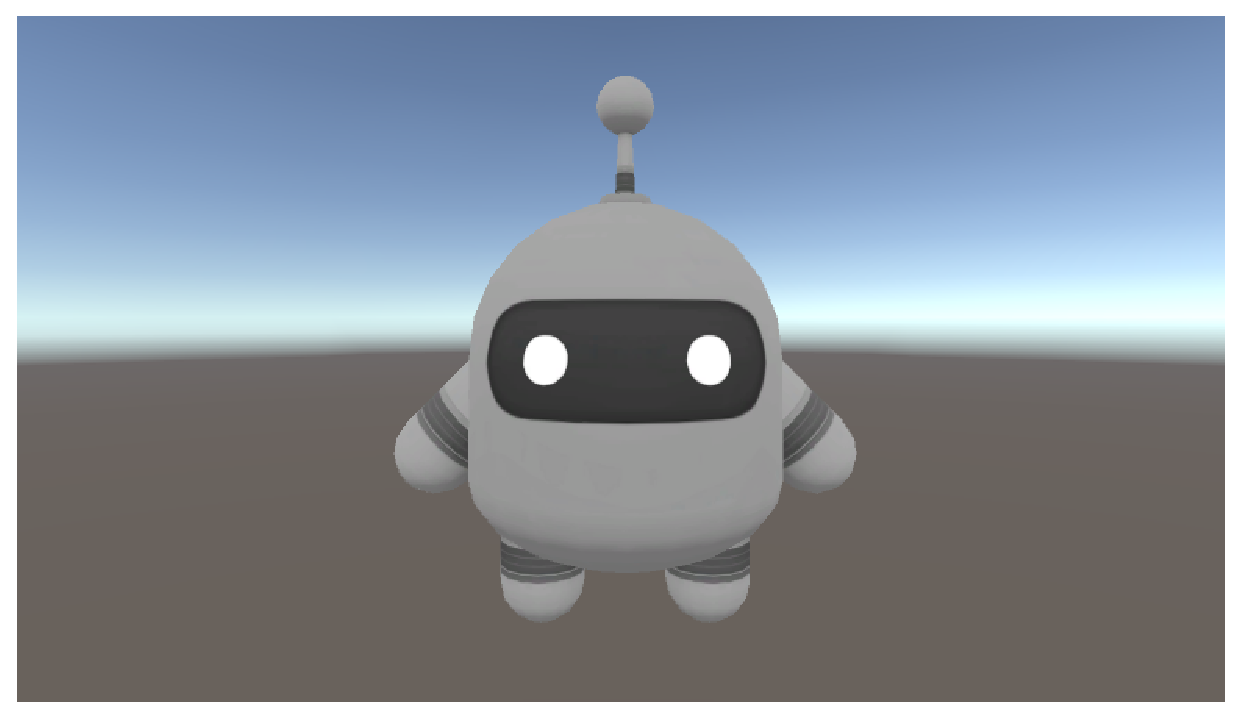
\includegraphics[width=12cm]{images/chapter3/Idle.eps}
  \caption{Idle状態のロボット}
  \label{Idle}
 \end{center}
\end{figure}

\vspace{1cm}
 \begin{figure}[!h]
 \begin{center}
  \centering
  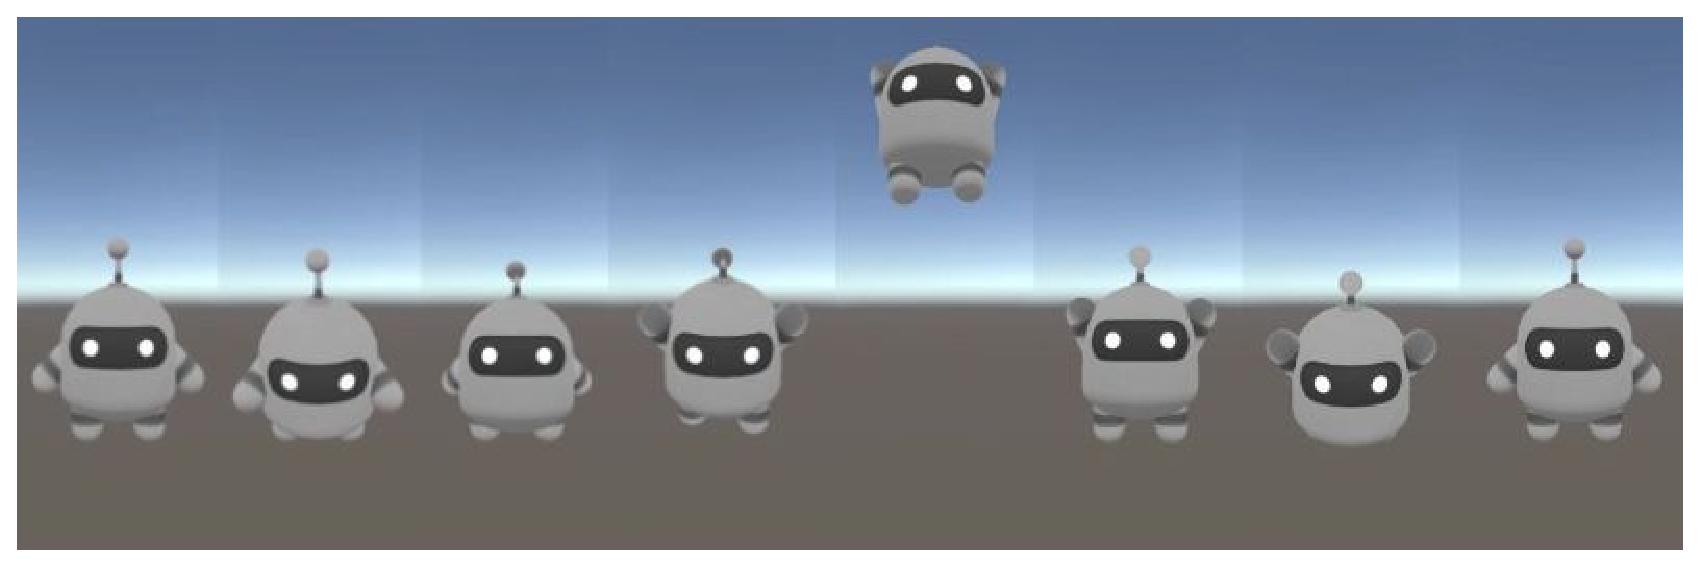
\includegraphics[width=12cm]{images/chapter3/happy.eps}
  \caption{喜の表出感情}
  \label{happy}
 \end{center}
\end{figure}

\vspace{1cm}
 \begin{figure}[!h]
 \begin{center}
  \centering
  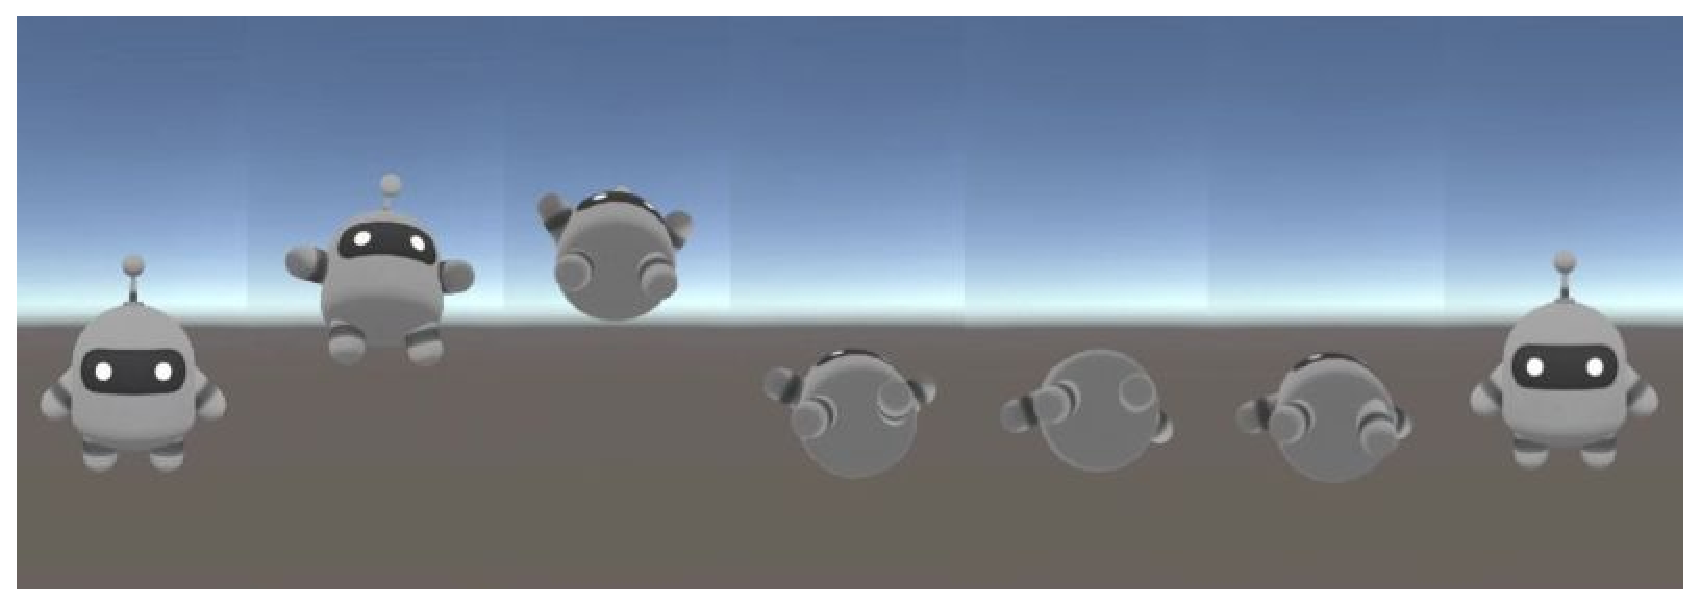
\includegraphics[width=12cm]{images/chapter3/sad.eps}
  \caption{哀の表出感情}
  \label{sad}
 \end{center}
\end{figure}

\newpage


















